Angenommen, wir testen die Ausprägung verschiedener Gene von 4 Mäusen und fassen die Ergebnisse in \zcref{tbl:intuitionpca} zusammen.
\begin{table}[tbh]
    \centering
    \caption{Datentabelle PCA}\label{tbl:intuitionpca}
    \begin{tabular}{lrrr}  
        \toprule  
        & Gen1 & Gen2 & Gen3 \\
        \midrule
        Maus 1 & 1,2 & 0,9 & 1,1 \\
        Maus 2 & 1,0 & 1,1 & 1,3 \\
        Maus 3 & 2,0 & 1,9 & 2,1 \\
        Maus 4 & 1,8 & 2,1 & 2,0 \\
        \bottomrule
    \end{tabular}
\end{table}
Dies können wir als dreidimensionalen Plot darstellen, indem ein Punkt je eine Maus repräsentiert.
\begin{figure}[h]
    \centering
    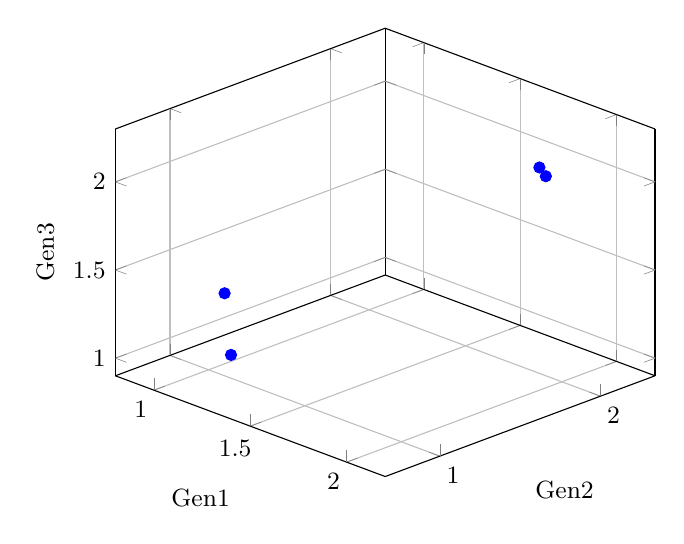
\begin{tikzpicture}
        \begin{axis}[
            view/h=45,
            grid=both,
            xlabel={Gen1},
            ylabel={Gen2},
            zlabel={Gen3},
            enlargelimits=0.2,
            tick label style={font=\small},
            label style={font=\small}
        ]
        \addplot3[only marks, mark size=2pt, color=blue] coordinates {
            (1.2, 0.9, 1.1)
            (1.0, 1.1, 1.3)
            (2.0, 1.9, 2.1)
            (1.8, 2.1, 2.0)
        };
        \end{axis}
    \end{tikzpicture}
    \caption{3D-Plot der Genexpressionen von vier Mäusen}
\end{figure}